\documentclass[a4paper, 11pt]{article}

% Packages
\usepackage[czech]{babel}
\usepackage[left = 2cm, top = 3cm, text={17cm, 24cm}]{geometry}
\usepackage{times}
\usepackage[T1]{fontenc}
\usepackage[utf8]{inputenc}
\usepackage{xcolor,listings}
\usepackage{hyperref}
\usepackage{url}
\usepackage{multirow}
\usepackage[ruled, linesnumbered, noline, longend]{algorithm2e}
\usepackage{graphicx}
\usepackage{pdflscape}
\usepackage{pict2e}
\SetNlSty{}{}{:}
\setlength{\algomargin}{3.25em}
\urlstyle{same}
\pagestyle{empty}

% Title page
\begin{document}
\begin{titlepage}
\begin{center}
\Huge
\textsc{Vysoké učení technické v~Brně}\\
\huge
\textsc{Fakulta informačních technologií}\\[0.4em]
\vspace{\stretch{0.382}}

\LARGE
Typografie a publikování\,--\,3. projekt\\
\Huge
Tabulky a obrázky\\
\vspace{\stretch{0.618}}

\Large
5.\,dubna 2021 \hfill Václav Valenta (xvalen29)
\end{center} 
\end{titlepage}

% Page 1
\thispagestyle{plain}
\clearpage

\section{Úvodní strana}
Název práce umístěte do zlatého řezu a nezapomeňte uvést dnešní datum a vaše jméno a příjmení.

\section{Tabulky}
Pro sázení tabulek můžeme použít buď prostředí\texttt{ tabbing }nebo prostředí\texttt{ tabular}.

\subsection{Prostředí\texttt{ tabbing }}
Při použití\texttt{ tabbing } vypadá tabulka následovně:

\begin{tabbing}
Vodní melouny\quad \= \bf Cena \quad \= \bf Množství
\quad \kill
	\bf Ovoce		\>\bf Cena	\>\bf Množství	\\[0.1em]
	Jablka			\>25,90	\>3 kg 		\\
	Hrušky		\>27,40	\>2,5 kg 		\\
	Vodní melouny	\>35,-- 	\>1 kus		\\
\end{tabbing}
\noindent
Toto prostředí se dá také použít pro sáyení algoritmů, ovšem vhodnější je použít prostředí\texttt{ algorithm } nebo\texttt{ algorithm2e } (viz sekce 3).

\subsection{Prostředí \texttt{ tabular}}

Další možnosti, jak vytvořit tabulku, je použít prostředí\texttt{ tabular}. Tabulky pak budou vypadat takto\footnote{Kdyby byl problém s\texttt{ cline }, zkuste se podívat třeba sem: \url{https://www.abclinuxu.cz/tex/poradna/show/325037}}:\\

\begin{center}\catcode`-=12
\begin{tabular}{|c|c|c|} \hline
	\multicolumn{1}{|c|}{} 	& \multicolumn{2}{|c|}{\bf Cena}	\\ \cline{2-3}
	\bf Měna			& \bf nákup 	& \bf prodej			\\ \hline
	EUR 				& 25,227 	& 26,943			\\ 
	GBP 				& 29,368 	& 31,492			\\ 
	USD 				& 21,260 	& 22,661			\\ \hline
\end{tabular}
\bigskip

Tabulka 1: Tabulka kurzů k dnešnímu dni
\bigskip\bigskip

\begin{tabular}{|c|c|}
\hline
	$A$ 	& $\neg A$ 	\\ \hline 
	\bf P 	& N 		\\ \hline
	\bf O 	& O 		\\ \hline 
	\bf X 	& X 		\\ \hline 
	\bf N 	& P 		\\ \hline
\end{tabular}
\begin{tabular}{|c|c|c|c|c|c|}
\hline
	\multicolumn{2}{|c|}{\multirow{2}{*}{$A \wedge B$}} 	& \multicolumn{4}{|c|}{$B$} 				\\ \cline{3-6} 
	\multicolumn{2}{|c|}{} 						& \bf P 	& \bf O 	& \bf X 	& \bf N 	\\ \hline
	\multirow{4}{*}{$A$} 				& \bf P 	& P 		& O 		& X 		& N 		\\ \cline{2-6} 
								& \bf O 	& O 		& O 		& N 		& N 		\\ \cline{2-6} 
	 							& \bf X 	& X 		& N 		& X 		& N 		\\ \cline{2-6}
	 							& \bf N 	& N 		& N 		& N 		& N 		\\ \hline
\end{tabular}
\begin{tabular}{|c|c|c|c|c|c|}
\hline
	\multicolumn{2}{|c|}{\multirow{2}{*}{$A \vee B$}} 		& \multicolumn{4}{|c|}{$B$} 				\\ \cline{3-6} 
	\multicolumn{2}{|c|}{} 						& \bf P 	& \bf O 	& \bf X 	& \bf N 	\\ \hline
	\multirow{4}{*}{$A$} 				& \bf P 	& P 		& P 		& P 		& P 		\\ \cline{2-6} 
								& \bf O 	& P 		& O 		& P 		& O 		\\ \cline{2-6} 
	 							& \bf X 	& P 		& P 		& X 		& X 		\\ \cline{2-6}
	 							& \bf N 	& P 		& O 		& X 		& N 		\\ \hline
\end{tabular}
\begin{tabular}{|c|c|c|c|c|c|}
\hline
	\multicolumn{2}{|c|}{\multirow{2}{*}{$A \rightarrow B$}} 	& \multicolumn{4}{|c|}{$B$} 				\\ \cline{3-6} 
	\multicolumn{2}{|c|}{} 						& \bf P 	& \bf O 	& \bf X 	& \bf N 	\\ \hline
	\multirow{4}{*}{$A$} 				& \bf P 	& P 		& O 		& X 		& N 		\\ \cline{2-6} 
								& \bf O 	& P 		& O 		& P 		& O 		\\ \cline{2-6} 
	 							& \bf X 	& P 		& P 		& X 		& X 		\\ \cline{2-6}
	 							& \bf N 	& P 		& P 		& P		& P 		\\ \hline
\end{tabular}
\end{center}

\noindent
Tabulka 2: Protože Kleeneho trojhodnotová logika už je \uv{zastaralá}, uvádíme si zde příklad čtyřhodnotové logiky\\

\bigskip
\pagebreak
\thispagestyle{plain}
\clearpage

\section{Algoritmy}
\noindent
Pokud budeme chtít vysázet algoritmus, můžeme použít prostředí\texttt{ algorithm }\footnote{ Pro nápovědu, jak zacházet s prostředí, algorithm, můžeme uźkusit tuhle stránku: \url{http://ftp.cstug.cz/pub/tex/CTAN/macros/latex/contrib/algorithms/algorithms.pdf}.}
nebo\texttt{ algorithm2e }\footnote{Pro\texttt{ algorithm2e } zase tuhle: \url{http://ftp.cstug.cz/pub/tex/CTAN/macros/latex/contrib/algorithm2e/doc/algorithm2e.pdf}. }.
Příklad použití prostředí\texttt{ algorithm2e }viz Algoritmus 1.\\

\smallskip
\begin{algorithm}[H]
\DontPrintSemicolon
\caption{\textsc{FastSLAM}}
\Indm	
	\KwIn{$(X_{t-1}, u_t , z_t)$}
	\KwOut{$X_t$}
\Indp
	$\overline{X_t} = X_t = 0$\;
	\For{$k = 1$ to $M$}{
		$x^{[k]}_t = sample\_motion\_model(u_t, x^{[k]}_{t-1})$\;
		$w^{[k]}_t = measurement\_model(z_t, x^{[k]}_t, m_{t-1})$\;
		$m^{[k]}_t = updated\_occupancy\_grid(z_t, x^{[k]}_t, m^{[k]}_{t-1})$\;
		$\overline{X_t} = \overline{X_t} + \langle x_x^{[m]}, w_t^{[m]} \rangle $\;
	}
	\For {$k = 1$ to $M$}{
		draw $ i $ with probability $\approx w_t^{[i]}$\;
		add $\langle x_x^{[m]}, w_t^{[m]} \rangle$ to $X_t$\;
	}
	\Return $X_t$
\end{algorithm}

\bigskip
\section{Obrázky}
Do našich článků můžeme samozřejmě vkládat obrázky. Pokud je obrázkem fotografie, můžeme klidně použít bitmapový soubor. Pokud by to mělo být nějaké schéma nebo něco podobného, je dobrým zvykem takovýto obrázek vytvořit vektorově.
\begin{center}
	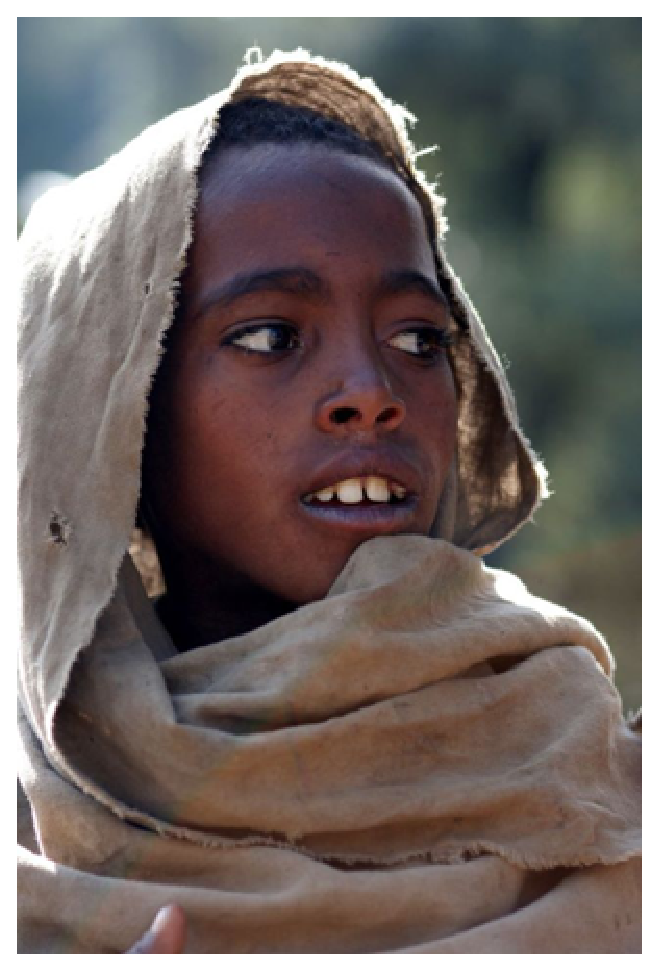
\includegraphics[scale = 0.4]{etiopan.eps}
	\reflectbox{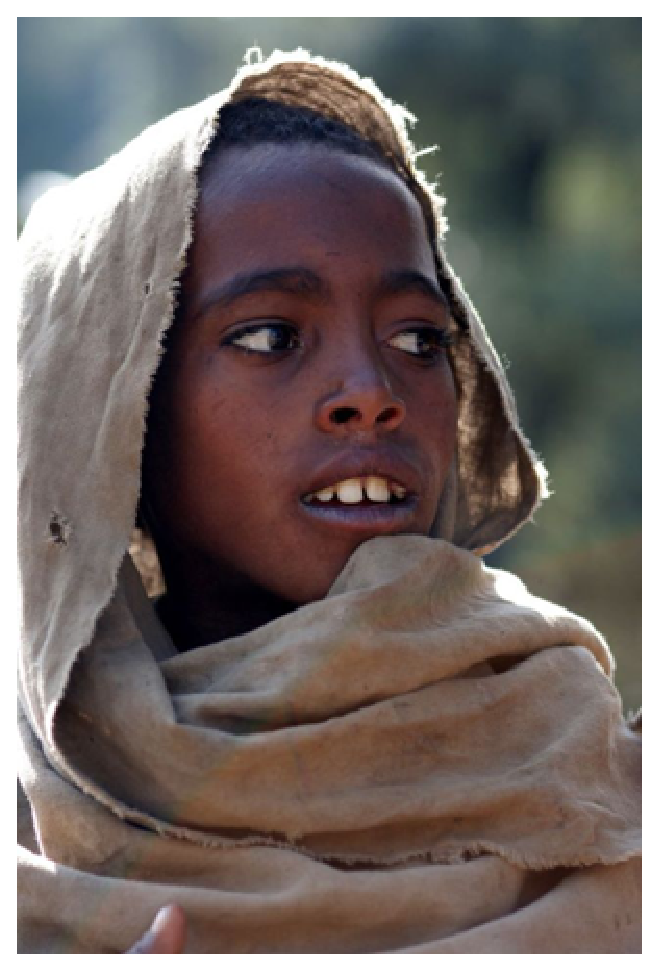
\includegraphics[scale = 0.4]{etiopan.eps}}\\
	Obrázek 1: Malý Etiopánek a jeho bratříček
\end{center}

\pagebreak
\thispagestyle{plain}
\clearpage

Rozdíl mezi vektorovým\dots\\
\begin{center}
	
\includegraphics[width=0.5\textwidth]{oniisan.eps}\\
	Obrázek 2: Vektorový obrázek
\end{center}
\smallskip
\dots a bitmapovým obrázkem\\
\begin{center}
	
\includegraphics[width=0.5\textwidth]{oniisan2.eps}\\
	Obrázek 3: Bitmapový obrázek
\end{center}

\bigskip \noindent
se projeví například při zvětšení.

Odkazy (nejen ty) na obrázky 1,2 a 3, na tabulky 1 a 2 a také na algoritmus 1 jsou udělány pomocí křížových odkazů. Pak je ovšem potřeba zdrojový soubor přeložit dvakrát.

Vektorové obrázky lze vytvořit i přímo v \LaTeX u, například pomocí protředí\texttt{ picture}.

\pagebreak
\clearpage
\thispagestyle{plain}
\begin{landscape}

\quad
\begin{center}
	\setlength{\unitlength}{1cm}	
	\begin{picture}(20,10)
		\put(0,0){\line(1,0){20}}
		\put(0,0){\line(0,1){10}}
		\put(20,10){\line(-1,0){20}}
		\put(20,10){\line(0,-1){10}}

	\setlength{\unitlength}{0.13cm}
		\put(49, 7){\line(1, 0){52}}
		\put(101, 7){\line(0, 1){36}}
		\put(49, 43){\line(0, -1){36}}
		\put(75, 69){\line(1, -1){30}}
		\put(75, 69){\line(-1, -1){30}}
		\put(45, 39){\line(-1, 1){2}}
		\put(43, 41){\line(1, 1){32}}
		\put(75, 73){\line(1, -1){32}}
		\put(105, 39){\line(1, 1){2}}
		\put(89, 59){\line(0, 1){10}}
		\put(89, 69){\line(1, 0){4}}
		\put(93, 69){\line(0, -1){14}}
		\put(89, 69){\line(0, 1){2}}
		\put(89, 71){\line(1, 0){4}}
		\put(93, 71){\line(0, -1){2}}
		\put(71, 7){\line(0, 1){18}}
		\put(71, 25){\line(1, 0){8}}
		\put(79, 25){\line(0, -1){18}}
		\put(53, 29){\line(0, -1){8}}
		\put(61, 21){\line(-1, 0){8}}
		\put(61, 21){\line(0, 1){8}}
		\put(61, 29){\line(-1, 0){8}}
		\put(57, 29){\line(0, -1){8}}
		\put(53, 25){\line(1, 0){8}}
		\put(63, 49){\line(0, -1){8}}
		\put(83, 41){\line(-1, 0){20}}
		\put(63, 49){\line(1, 0){20}}
		\put(83, 49){\line(0, -1){8}}
		\put(73, 41){\line(0, 1){8}}
		\put(83, 45){\line(-1, 0){20}}
		\put(63, 51){\line(1, 1){10}}
		\put(73, 61){\line(1, -1){10}}
		\put(83, 51){\line(-1, 0){20}}
		\put(81, 51){\line(-1, 1){8}}
		\put(73, 59){\line(-1, -1){8}}
		\put(87, 29){\line(0, -1){8}}
		\put(87, 21){\line(1, 0){8}}
		\put(95, 21){\line(0, 1){8}}
		\put(95, 29){\line(-1, 0){8}}
		\put(91, 29){\line(0, -1){8}}
		\put(87, 25){\line(1, 0){8}}
		\put(130,60){\circle{8}}            
           \end{picture}\\
	Obrázek 4: Vektorový obrázek útulného rodinného domku
\end{center}

\end{landscape}
\end{document}